\section{The HARP framework}

In this Section, firstly, a brief overview of the HARP framework for graph coarsening \cite{chen_harp_2018} is presented, followed by our analysis of the properties of graph coarsenings in general.

\subsection{HARP}\label{sec:harp}
HARP is a method for improving the performance of graph representation learning (i.e. graph embedding) algorithms such as DeepWalk \cite{perozzi_deepwalk_2014}, LINE \cite{tang_line_2015}, PTE \cite{tang_pte_2015} or node2vec \cite{grover_node2vec_2016}. The method is a combination of dataset augmentation and pre-training based on the general principle that graph-based models train more efficiently on smaller graphs and can thus be pre-trained on a coarsened representation of the graph at hand. Moreover, the coarsened graphs are able to approximate the global properties of the original data, enabling the representations to better encapsulate such a global structure. In an overview, the method consists of the following steps:

Consider an undirected graph \( G \) with nodes \( V \left( G \right) \) and edges \( E \left( G \right) \). The aim of the graph coarsening part of the algorithm is to generate a sequence of graphs \( G_0, G_1, G_2, \dots, G_L \) where \( G_0 = G \) and \( L \in \mathfield{N} \) is a hyper-parameter of the method. In this sequence, each graph \( G_i \) is generated from the graph \( G_{i - 1} \) by coarsening it -- lowering the number of nodes and edges while preserving in some sense the general structure of the graph. Following \cite{chen_harp_2018}, let \( \psi_i \) denote the mapping of the vertices of \( G_{i - 1} \) such that \( V \left( G_i \right) = \psi_i \left( V \left( G_{i - 1} \right) \right) \).

\begin{enumerate}
  \item \textbf{Dataset augmentation}. The graph \( G \) is consecutively reduced in size by the application of several graph coarsening schemas. In each step, the coarsened graph can be viewed as an ever coarser representation of the graph data and its global structure. This step can be run ahead-of-time to produce the resulting coarsened graphs \( G_0, G_1, \dots, G_L \).
\end{enumerate}
After all the coarsened graphs are pre-computed, the method itself can be executed by repeating the following steps on the graphs from the coarsest to the finest (i.e. from \( G_L \) to \( G_0 \)):
\begin{enumerate}\setcounter{enumi}{1}
  \item \textbf{Training on an intermediary graph}. The graph embedding model is trained on \( G_i \), producing \( \Phi_{G_i} \), an embedding of the graph in an Euclidean space.
  \item \textbf{Embedding prolongation}. The embedding \( \Phi_{G_i} \) is prolonged from the current graph to one that is one step closer to \( G_0 \), yielding \( \Phi_{G_{i - 1}} \). This embedding is used as the starting state for training on \( G_{i - 1} \).
\end{enumerate}
These steps are repeated until \( \Phi_{G_0} \) is computed. While the training step of this schema is a straightforward application of one of the aforementioned embedding algorithms to \( G_i \), the particular details of the coarsening and prolongation steps are further explained in Sections \ref{sec:adaptive-prolongation} and \ref{sec:harp-coarsening}.

The first step is independent of the rest of the computation and can be done ahead of time. The last two steps can be seen as a form of pre-training for the model that is to be learnt on the original graph. The whole HARP pipeline is demonstrated in Figure \ref{fig:harp-overview}.\todo{The image isn't exactly correct}

\begin{figure}
  \centering
  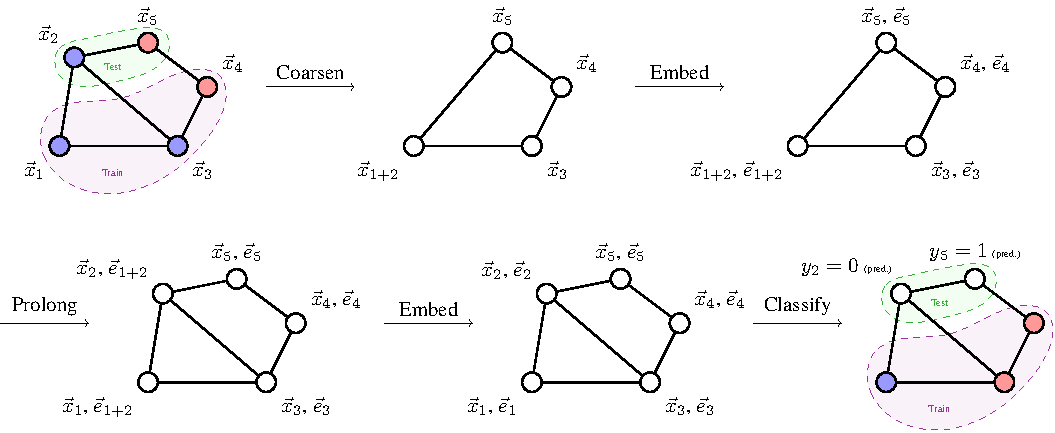
\includegraphics[width=\linewidth]{images/harp-overview/harp-overview.pdf}
  \caption{An overview of the HARP processing pipeline with one level of coarsening}
  \label{fig:harp-overview}
\end{figure}

\subsection{Properties of graph coarsenings}\label{sec:coarsening-properties}

The HARP framework presents a particular way of producing coarsened graphs. In general, however, we would like to describe any coarsening of a graph in order to be able to explore the set of all coarsened graphs to study the properties of both the applied algorithms, as well as the underlying data.

To properly describe the set of all coarsenings, some assumptions are made about what constitutes a coarsening. In our work, we define a coarsening as a set \( \mathcal{C} \subseteq E \left( G \right) \), i.e. a subset of edges of the original graph. The graph \( H = \varphi_\mathcal{C} \left( G \right) \) obtained by applying this coarsening to \( G \) is constructed from \( G \) by contracting all edges in \( \mathcal{C} \)\footnote{Whether to allow parallel edges to arise from this operation is left to the user.}. This description of a graph coarsening is inspired and builds upon the work \cite{schulz_mining_2019}, which is why it differs from the weaker definition of a graph reduction as selecting a subset of nodes and edges.\todo{Martine, tady navrhuješ nějaké citace, ale 2 z nich jsem nenašel.}

Under such a definition of a graph coarsening, the set of all coarsenings of a graph \( G \) forms a complete bounded lattice with the partial order
\[ \varphi_{\mathcal{C}_1} \preceq \varphi_{\mathcal{C}_2} \iff \mathcal{C}_1 \subseteq \mathcal{C}_2 \]
The least element (bottom) of this lattice is the coarsening \( \bot = \varphi_\emptyset \) where \( \bot \left( G \right) = G \). The greatest element (top) of this lattice is the coarsening \( \top = \varphi_{E \left( G \right)} \), where \( \top \left( G \right) \) is a graph in which there is a single node for each connected component in \( G \). In ideal conditions, to study the effect of graph coarsenings on its quality (viewed through the lens of a downstream task), one would exhaustively study this lattice. In practice, such an exhaustive search is computationally infeasible. With a method such as HARP, one can view the coarsened graphs produced by the method as a kind of \enquote{path} through the set of all coarsenings - the individual coarsenings represent one way of navigating the lattice with them forming a chain between \( \top \) and \( \bot \).
